\documentclass[a4paper,12pt]{report}
\usepackage[english]{babel}
\usepackage{amsmath}
\usepackage{graphicx}
\usepackage{lscape}
\usepackage{rotating}
\usepackage{longtable}
%\usepackage[authoryear]{natbib}
\usepackage[numbers]{natbib}
\usepackage{hyperref}
\usepackage{subfig}
\usepackage{url}
\begin{document}
\title{MSc Thesis - Benchmark of {\em De Novo} Short Read Assembly Strategies for Metagenomics}
\author{Ino de Bruijn\\ {\bf Supervisor:} Assistant Prof. Anders Andersson}

\maketitle

\tableofcontents

\chapter{Introduction}
% random comment
Metagenomics, the sequencing of environmental DNA, has demonstrated to be a
promising approach for the discovery and investigation of microbes that cannot
be cultured in the laboratory \cite{Eisen17355177} as well as for the study of
both free-living microbial communities \cite{Andersson18497291} and microbial
communities inside other organisms \cite{Qin20203603,Hess21273488}.\\


In a typical shotgun metagenomics experiment the DNA of a community is isolated
and high throughput sequencing is performed on a random sample of the isolated
DNA \cite{Morgan20419134}. The reads can either be analyzed as such, by e.g.
blast searches against reference databases to obtain a functional profile of
the microbial community \cite{Tringe15845853}, or they can be assembled to form
longer stretches of DNA stemming from the same or closely related organisms
that can subsequently be analyzed with regards to phylogenetic affiliation and
functional properties. The output of the assembly process often includes
scaffolds, contigs and unassembled reads \cite{Mavromatis17468765}. One of the
problems with assembling is that chimeric contigs or scaffolds may be formed.
Closely related sequences are more likely to form chimeras and since closely
related strains often occur in the same environment this is a challenge. Also,
it is difficult to determine whether the formation of a chimera is natural due
to homologous recombination or an error in the assembly process
\cite{Tyson14961025}. Another problem with assembly is variations in gene
content among closely related strains, since a gene inserted in a subpopulaton
will cause conflicting assembly results \cite{Hallam17114289}. After assembling
the reads, a process called binning is performed, where the resulting scaffolds
and contigs are assigned to phylogenetically related groups. Finally, gene
calling and functional annotations are performed on the scaffolds.\\

% rewrite upper part (maybe take some parts from theoretical background)

In our studies several strategies for {\em de novo} assembly of metagenomics
have been evaluated. Illumina short read libraries have {\em in silico} been
shown to work well on communities of medium complexity \cite{Mende22384016},
therefore we have chosen to assess the assembly strategies for Illumina paired
short reads sepecifically. In previous studies mostly {\em in silico}
metagenomic data sets have been used
\cite{Pignatelli21625384,Mavromatis17468765}. In contrast the community of our
study is an {\em in vitro} simulated metagenome consisting of 59 species with
completed or nearly completed genomes so the quality of our assesment is not
dependent on the realisticness of read simulators. An even and uneven
distribution of the 59 species were created in vitro. The community has been
sequenced with different type of library preparations to be able to test the
difference in library preparation as well.  The following assembly programs
have been tested: Velvet \cite{Zerbino18349386}, Meta-Velvet \cite{MetaVelvet},
Newbler \cite{Quinn18755037}, Minimus2 \cite{Sommer17324286}, Ray Meta
\cite{Boisvert23259615} and Bambus2 \cite{Koren21926123}. The quality of the
assemblies have been evaluated by mapping the constructed contigs or scaffolds
to the collection of reference genomes, hereafter referred to as the reference
metagenome. In addition two pipelines have been constructed, one to perform the
assemblies and another to perform the validation given there is a reference
metagenome available.

%\chapter{Theoretical Background}
%% maybe mention some general paper overview of different assembly methods
%% PRactical ZHang de novo genome assembly).
%%Studying microbes in their natural environment is difficult for a number of reasons. One obvious
%%reason is that their size makes field studies impractical. A way around this
%%issue is culturing microbes in the laboratory. Unfortunately the vast majority of
%%microbes have not successfully been cultured in the lab \cite{Eisen17355177}.
%%By isolating the DNA of a community and sequencing that, analysis of a
%%community $in vivo$ can be performed. The most popular methods for sequencing
%%DNA from a sample of microbes are Illumina paired end and 454 sequencing (TODO:
%%citations). The sequencing process results in short reads of around 100 bp for
%%Illumina HiSeq and around 400 bp up to 1 kbp for 454 GS FLX Titanium (TODO:
%%citations). After sequencing the reads can be mapped against a reference
%%database of the same or closely related organisms to get a functional profile
%%of the community. Assembling the reads into longer contiguous segments of DNA
%%(contigs) before functional analysis has however been shown to improve the
%%accuracy (TODO: citations). 
%
%
%There are mainly three different categories of assembly approaches:
%Greedy-extension, de Bruijn graph and Overlap-Layout-Consensus (OLC)
%\cite{Zhangdadad}. Greedy-extension is a string-based method and the latter two
%use graphs.

\chapter{Related Work}
% Start with success of single genome evaluation, continue to metagenomic

In a study by \citet{Mavromatis17468765} three genome assemblers were
evaluated: Phrap \cite{delaBastide18428783}, Arachne \cite{Batzoglou11779843}
and Jazz \cite{Aparicio12142439}. For the evaluation three artificial
communities were constructed of low, medium and high complexity by selecting
Sanger reads from 113 isolate genomes. The low complexity community had one
dominating population with several low-abundance ones, the medium more than one
dominating population and the complex community had no dominating population at
all. Resulting contigs were evaluated on chimericity and length distribution.
Compared to using the original reads for gene annotation, assembly was
demonstrated to give not more than 20\% increase in accurate gene prediction
and a slightly better increase for inaccurate and missed genes, however 700 bp
long Sanger reads were used in this study. This approach of using artificial
communities has subsequently been used in adapted versions by several other
assembly evaluation papers \cite{Pignatelli21625384,Mende22384016}. In the
benchmark by \citet{Pignatelli21625384} the reads of the artificial communities
were changed from Sanger to 454 and Illumina. For the Illumina reads, SSAKE
\cite{Warren17158514} and Velvet were used to perform the assembly.  No
difference in chimericity between using the simulated 454 reads or the Illumina
reads was spotted. The main cause of chimericity was sequence similarity of the
organisms, no relation with genome coverage was found. At the functional level
metagenomic assembly turned out to be counterproductive compared to using the
original reads for annotation. \citet{Mende22384016} used a metagenome of 10,
100 and 400 species with simulated reads of Illumina, 454 and Sanger with
sequencing depth based on sequencing cost for each technology. All of the
technologies provided similar coverage for 10 species. Illumina was superior
for 100 species due to the higher coverage one can get for a similar price.
Sanger performed best for 400 species because of longer read length. Sanger
reads were assembled with Arachne; 454 reads with Celera \cite{Myers10731133}
and Illumina reads with SOAPdenovo \cite{Li20019144}. In contrast to the study
of \citet{Pignatelli21625384} a year earlier, contigs now did turn out to
improve functional annotation of the metagenome. Furthermore using Illumina
paired end data to determine contig links and construct scaffolds, although
introducing more chimerism, resulted in an even better functional annotation.
Beyond using simulated reads or real reads of {\em in silico} communities
there has not been a comparison of assembly algorithms using an {\em in vitro}
community yet.  In vitro communities have been used previously with success to
assess DNA extraction techniques for sequencing a low complexity community of
nine bacterial genera \cite{Willner22514642}, an oral community
\cite{Diaz22520388}, the human gut \cite{Wu20673359} and the human microbiome
\cite{HMPC22699610}.  The advantage of using an {\em in vitro} community for
assembly evaluation is that one does not have to rely on the correctness of
sequencing simulators, the assessment can thus be as good as the similarity of
the {\em in vitro } community to a real community.

%Say something about GAGE and Assemblathon

\chapter{Methods and Materials} To determine the quality of metagenomic assembly a mock
community of species with known genomes was constructed {\em in vitro} and
sequenced with Illumina. The resulting reads have been assembled using a
combination of Velvet, Meta-Velvet, Ray, Minimus2, Newbler and Bambus2 resulting in
nineteen different assembly strategies (see Figure \ref{fig:asmstrat} and Table
\ref{tab:asmstrat}). The strategies stem from current literature and our own
ideas.

\section{Mock community} The mock community consists of 49 bacterial and 10
archaeal species with finished or nearly completed genomes (Table
\ref{tab:mock}). The species have been chosen such that there are a number of
closely related organisms and more distant ones. The number of species is about
equal to the number of species one would find in the human gut. The abundances
of DNA from each species have been fixed in two types of configurations before
sequencing. In the first configuration, the even configuration, all species
have approximately equal genome copy numbers. In the second configuration, the
uneven configuration, the phyla are mixed in proportions similar to log-normal
distributions of phyla in soil \cite{Doroghazi18682841}. The samples have been
prepared with the Nextera 50ng sample preparation kit. The entire reference
metagenome's size is about 195Mb. 

% The V3 (192 bp) and V4 (291 bp) of the 16S genes have been amplified and the samples have been sequenced with Illumina.

\section{Quality trimming} Before assembling the reads one often starts with
pre-processing them by quality trimming and/or removing PCR duplicates.
\citet{Mende22384016} demonstrated that quality trimming could drastically
improve the assembly. Before each assembly the same quality trimming procedure
has been performed. For quality trimming the program sickle was used (see Table
\ref{tab:programversions}). Reads were trimmed from the 3' end if the average
quality score was below 20 in a window of 10 bases.


\section{Assembly} In the assembly procedure reads are combined into
contiguous sequences called contigs. Contigs can afterwards be joined using
paired read information into longer scaffolds. In the scaffolding process
contigs might be extended and repeats might be solved so scaffolding is not
restricted to just the ordering of contigs.\\


There are a plethora of different assemblers available and by pre-processing
reads and combining different assemblers an even larger amount of assembly
strategies is possible. Velvet is one of the most used assembly programs and
was therefore included in this assessment. Velvet's metagenomic counterpart,
Meta-Velvet, is performed after executing Velvet so it is possible to determine
how the metagenomic specific parameters improve the assembly. Another popular
assembler that has recently received an update for metagenomics is Ray (TODO:
cite). Ray is based on MPI and is runnable over multiple nodes distributing
both memory and processor load, which makes it an ideal candidate for large
metagenomic projects.\\


\subsection{Contiging}
Velvet, Ray and Meta-Velvet all use a de Bruijn graph to determine overlaps
between reads. This involves cutting up the reads in sizes of a specified kmer
size and let edges represent overlaps between kmers. This way the graph, or the
computational requirements, grow with the number of unique kmers in the library
instead of the number of reads. For a more elaborate description of de Bruijn
Graphs for sequence assembly see \cite{Miller20211242}. The resulting contigs
are constructed by following paths in the graph. The paths that can be
unambiguously followed are called unitigs. Ambiguous paths can be solved by
using coverage information or paired-end information. Contigs thus consist of
one or multiple unitigs. Choosing the right kmer size is important. A shorter
$k$ gives more coverage but at the same time the risk increases that the kmer
occurs multiple times within the genome, or in multiple genomes. A larger $k$
can overcome this problem if it is larger than the multiply occurring region,
thereby creating unique kmers instead of one kmer with more coverage.\\


\subsubsection{How the assemblers differ}
Velvet, Ray and Meta-Velvet differ in the way the graph is traversed. Velvet,
meant for single genomes, looks for one coverage peak in the coverage
distribution and tries to follow that, where the main idea is that the genome
is approximately uniformly covered. Nodes in the graph below a certain coverage
threshold are considered errors and ones with high coverage repeats.
Meta-Velvet looks for multiple peaks in the coverage distribution. Each genome
should have a distinct coverage peak due to its genome copy number and genome
length being different from the other genomes in the metagenome. Meta-Velvet
makes use of that property. Ray looks for 'seeds' in the graph and extends
those seeds iteratively weighting choises by the number of reads supporting a
certain path. The seeds are unitigs in the graph with a specific coverage. The
metagenomic update to Ray changes the seed selection by looking at the coverage
peak in the graph locally instead of globally. 


\subsection{Merging}
A way to get the advantage from both short and long kmers is by merging contigs
generated in multiple assemblies with different kmer lengths. This is possible
with Newbler, as done by \citet{Luo22347999}, or with Minimus2, as done by for
instance the Rnnotator pipeline \cite{Martin21106091}. Both Newbler and
Minimus2 use an Overlap-Layout-Consensus method to merge contigs
\cite{Sommer17324286,Miller20211242}.


\subsection{Scaffolding}
For the scaffolding procedure Bambus2 was chosen since it was one of the better
scaffolders for single genomes in the GAGE assessment paper
\cite{Salzberg22147368} and is suitable for metagenomes as well
\cite{Koren21926123}. For a flow diagram of previously mentioned approaches see
Figure \ref{fig:asmstrat}. A total of twelve assembly strategies from the flow
diagram have been tested. See Table \ref{tab:asmstrat} for an overview of the
assembly strategies, Table \ref{tab:programversions} for versions of each
program and Table \ref{tab:asmstratparameters} for the parameters of each
strategy.


\begin{table}[h!]
\centering
\begin{tabular}{|l|c|c|c|}
\hline
Assembly strategy name & Contiging & Merging & Scaffolding\\
\hline
velvetnoscaf & Velvet & - & -\\
velvetscaf & Velvet & - & Velvet\\
minimus2velvetnoscaf & Velvet & Minimus2 & -\\
newblervelvetnoscaf & Velvet & Newbler & -\\
bambus2velvetnoscaf & Velvet & - & Bambus2\\
bambus2minimus2velvetnoscaf & Velvet & Minimus2 & Bambus2\\
bambus2newblervelvetnoscaf & Velvet & Newbler & Bambus2\\
metavelvetnoscaf & Meta-Velvet & - & -\\
metavelvetscaf & Meta-Velvet & - & Meta-Velvet\\
minimus2metavelvetnoscaf & Meta-Velvet & Minimus2 & -\\
newblermetavelvetnoscaf & Meta-Velvet & Newbler & -\\
bambus2metavelvetnoscaf & Meta-Velvet & - & Bambus2\\
bambus2minimus2metavelvetnoscaf & Meta-Velvet & Minimus2 & Bambus2\\
bambus2newblermetavelvetnoscaf & Meta-Velvet & Newbler & Bambus2\\
raynoscaf & Ray & - & -\\
rayscaf & Ray & - & Ray\\
minimus2raynoscaf & Ray & Minimus2 & -\\
newblerraynoscaf & Ray & Newbler & -\\
\hline
\end{tabular}
\caption{Assembly strategies}
\label{tab:asmstrat}
\end{table}

\clearpage
\thispagestyle{empty}
\begin{figure}[ht!]
  \centering
    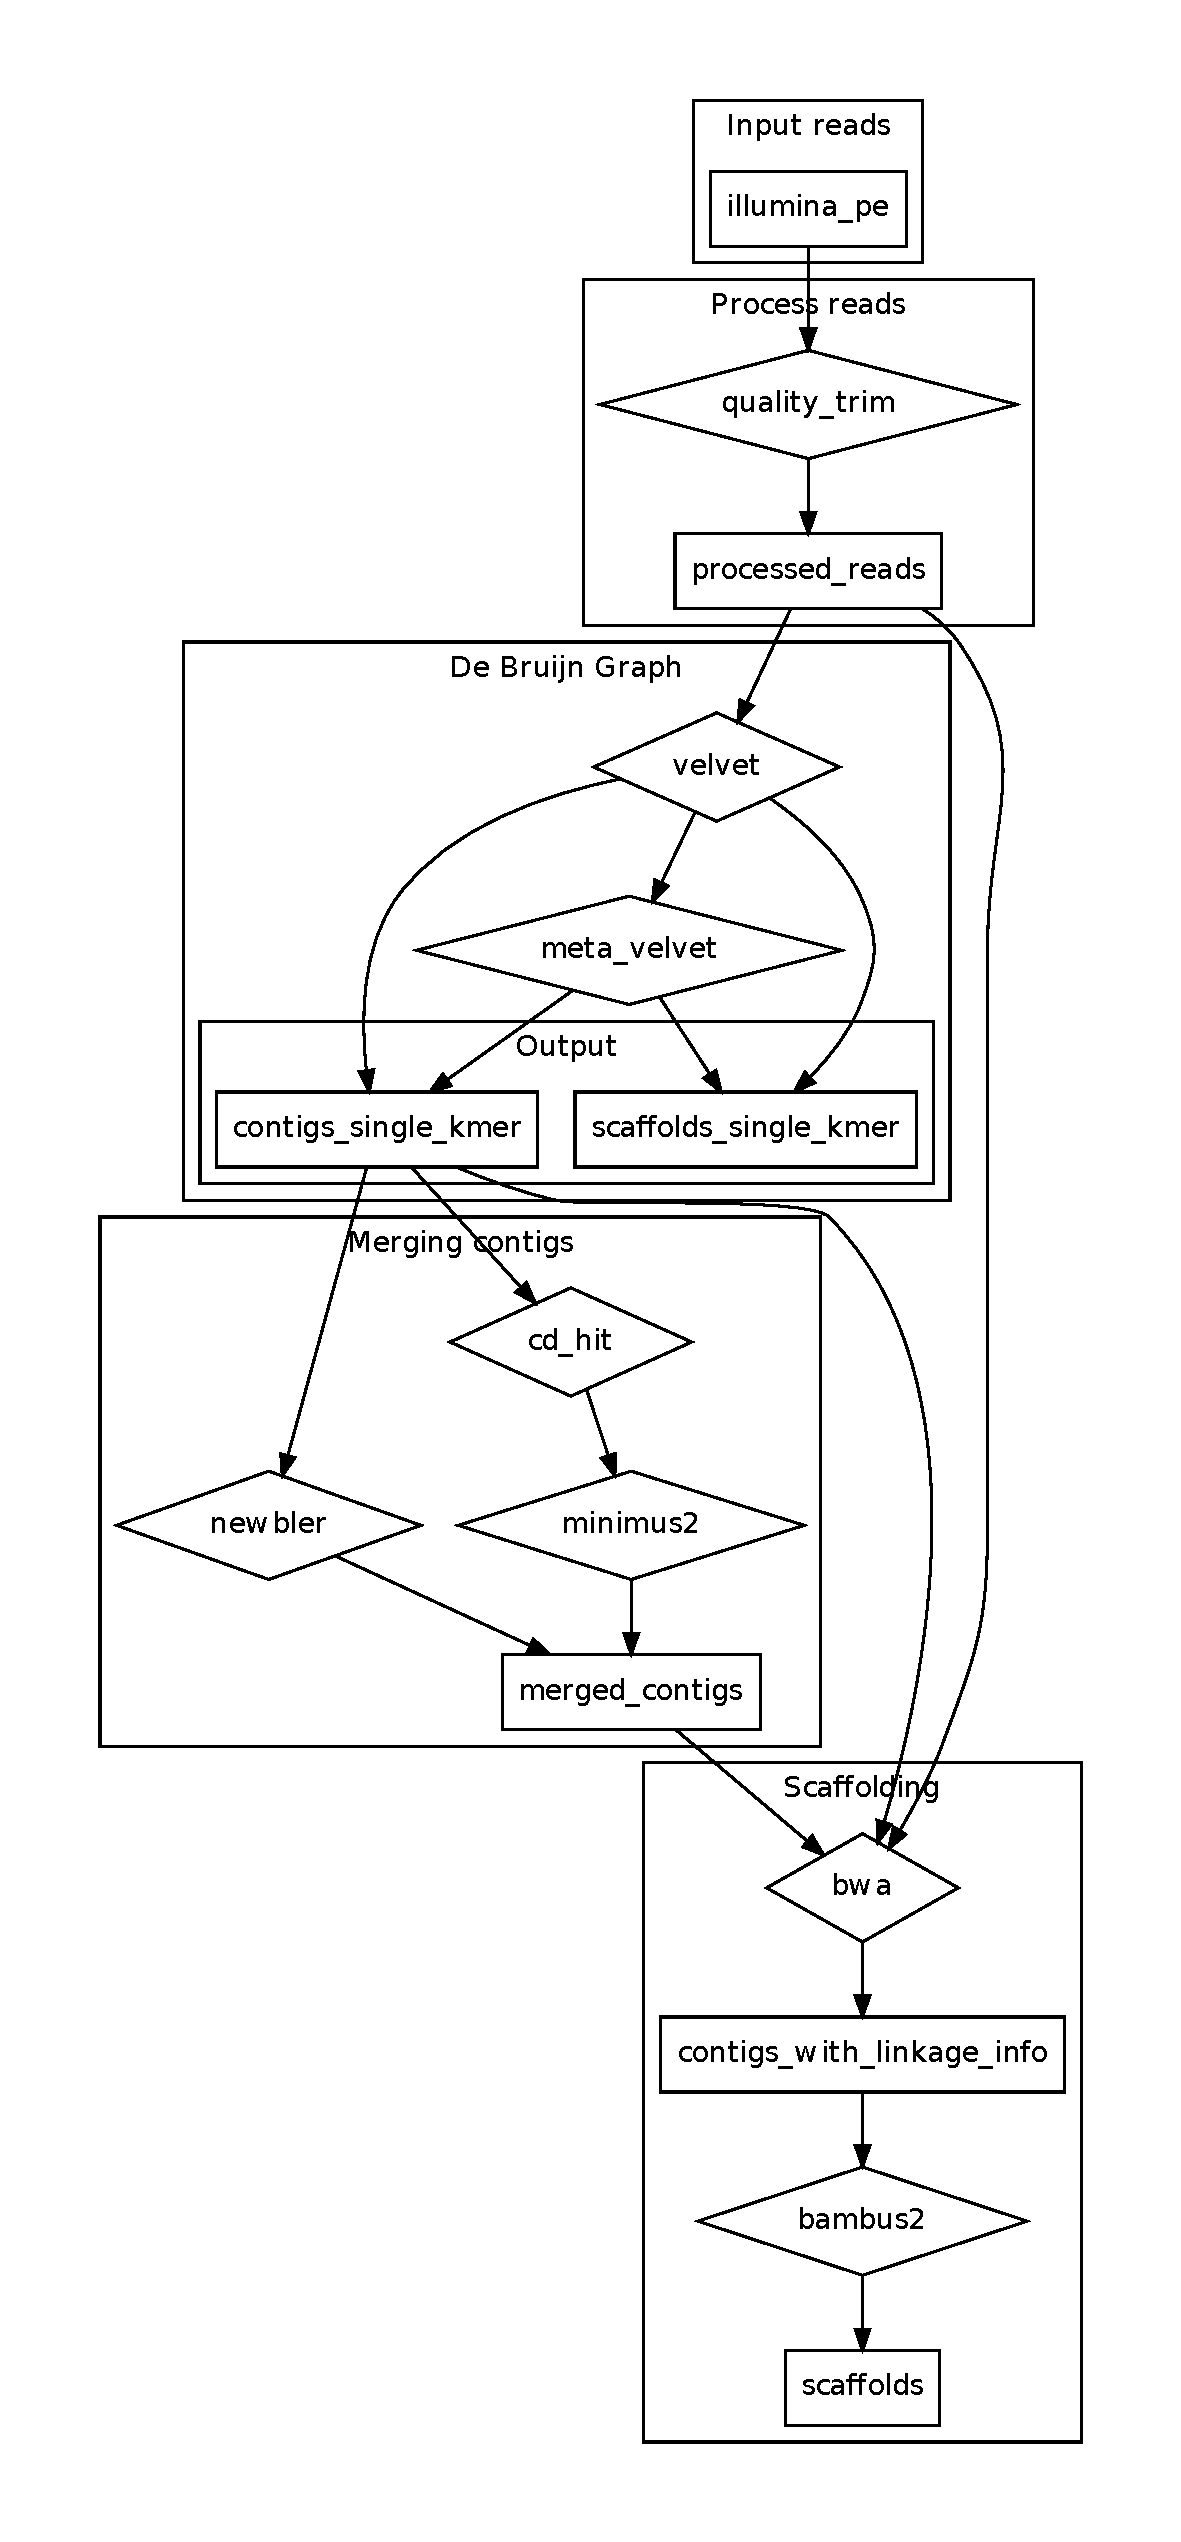
\includegraphics[height=\textheight]{figures/metassemble-flowchart.pdf}
  \caption{Assembly strategies using a combination of Velvet, Meta-Velvet, Ray, Minimus2, Newbler and Bambus2.}
  \label{fig:asmstrat}
\end{figure}

%TODO Validation requires some more non-ambiguous parameters for calculating
% the statistics and performing the mapping with MUMmer

\clearpage \section{Validation} \label{sec:metval} The validation of a metagenomic assembly in
case a reference metagenome is available often focuses on one or more of the
following points:
\begin{itemize}
\item contig or scaffold length distribution
\item chimericity of the contigs/scaffolds
\item contig/scaffold coverage of the reference metagenome
\item functional annotation
\item phylogenetic classification
\end{itemize}
This study focusses on the first three points, since those are expected to
improve the functional annotation and the phylogenetic classification.
\citet{Mende22384016} showed that this was indeed the case for functional
annotation.\\


A variety of metrics are used in this validation. For the contig/scaffold
length distribution of an assembly a common metric called the L50 value is
used. L50 is a median value weighted by contig length. Half of all the bases in
the assembly is in contigs equal to or larger than L50. For determining how
well the assemblies matched the reference metagenome the assemblies were mapped
against the reference metagenome using MUMmer 3.1 \cite{Kurtz14759262}.  MUMmer
finds maximal exact matches longer than $l$ and clusters them if they are no
more than $g$ nucleotides apart. The alignments are afterwards extended for
each cluster if the combined length of its matches is at least $c$. The
alignments are extended in between the matches of the cluster and on the ends
using a Smith-Waterman dynamic programming algorithm. The MUMmer package
contains multiple scripts that make use of this approach. NUCmer
(\underline{NUC}leotide MUM\underline{mer}) is a script included in the MUMmer
package for DNA sequence alignment of a set of query contigs against a set of
reference contigs. The command for NUCmer used was: 
\verb!nucmer --maxmatch -c65 -g90 -l20!. The maxmatch parameter makes sure all
exact matches are used, whether they are unique or not, so contigs that consist
only of a shared region or a repetitive element will be included in the
alignments as well. Afterwards the script \verb!show-coords! was used on the
resulting alignment file to extract information about each alignment such as
its location in both the query and the reference, percent identity, percent
similarity and percent of the reference and query covered.\\


In previous research by \citet{Mavromatis17468765} chimericity of
each contig was determined by the reads mapping to it. This could be done
because reads were selected from finished genome projects, thus 
the origin of each read is known. At each taxonomic level from strain to domain the
contigs were assigned to the phylogenetic group where the majority of reads
stem from. The chimericity was then defined as the number of
reads that belong to another phylogenetic group divided by the total number of
reads mapping to the contig.  \citet{Mende22384016} noted that certain
reads might actually belong to multiple species since there are shared regions between species.
Therefore they proposed a metric called contig score, which is determined by mapping
each contig with blastn to the original genomes, taking the Highest Scoring
Segment Pair (HSP) and multiplying the percent identity times the percent
contig coverage. We use a similar metric, determined with MUMmer
and referred to as purity instead to indicate its relation to chimericity. For
each alignment the purity $p$ is determined by multiplying percent contig
coverage by percent identity divided by 10,000 to get the purity as a ratio
between 0 and 1. The purity of a contig is the maximum purity of all its
alignments. Purity of an entire assembly is computed as well. If $n$ is the
number of contigs, $l_1,...,l_n$ the length of each contig in nucleotides and
$p_1,...,p_n$ the purity of each contig then purity $P$ of an entire
assembly is calculated as:

\begin{equation}
P = \frac{\sum_{i=1}^n l_{i} * p_{i}}{\sum_{i=1}^{n} l_{i}}
\end{equation}

For both scaffolds and contigs, only nucleotides are counted when determining
$l$.\\


To indicate how well the metagenome is covered by the assembled contigs we use
a metric called genome contig coverage and metagenome contig coverage. For each
genome in the reference metagenome, genome contig coverage is determined by
dividing the number of bases that are covered by contigs mapping to it by the
total number of bases in the genome. Metagenome contig coverage is the number
of bases covered by all contigs mapping to it divided by the total number of
bases in the metagenome. In both cases only the best alignment for each contig
based on previously described purity metric are considered. In case a contig
aligns equally well to multiple locations, all alignments are considered. This
can for instance be the case for a contig that represents a repeat or a shared
region between genomes.

\subsection{Pipeline} The vast amount of assemblies that had to be performed
gave rise to a need for automation. The pipeline had to be robust to errors
because the assembly programs often suffer from unexpected crashes for
different libraries. One would prefer to have assemblies not depended on a
previously crashed assembly to execute anyway. That way the user can decide
whether spending time on fixing the error for that assembly and the dependent
assemblies is worthwhile. Another important aspect was that the assemblies had
to be reproducible otherwise an evaluation is of very little use to the
scientific community. A pipeline called MetAssemble has been developed in GNU
Make for Illumina paired reads. All assemblies can be done in one go or a
specific assembly can be performed. It is also possible to only get the
commands for a specific assembly by doing a dry-run so one can easily create
their own scripts.

\chapter{Results}
All assemblies in Table \ref{tab:asmstrat} have been performed on the
following libraries:
\begin{description}
\item[50ng even] Community prepared with 50 ng Nextera library prepartion kit and equal
genome copy numbers. The library has been sequenced with Illumina and contains
$\sim$10M paired reads, each single read has a length of 100.
%\item[500pg even] Community prepared with 500 pg Nextera library prepartion kit and equal
%genome copy numbers.
\item[50ng uneven] Community prepared with 50 ng Nextera library prepartion kit
and phyla mixed similar to log-normal distributions of phyla in soil. The
library has been sequenced with Illumina and contains $\sim$10M paired reads,
each single read has a length of 100.
%\item[500pg uneven] Community prepared with 500 pg Nextera library prepartion kit and phyla
%mixed similar to log-normal distributions of phyla in soil.
\end{description}

The original reads of each library were mapped against the reference genome
using BWA \cite{Li20080505} and default values. Afterwards duplicates were
removed with MarkDuplicates from Picard 1.77 (see also Table
\ref{tab:programversions}). In Figure \ref{fig:coverage50ngeven} the even
spread of the coverage for the even library can be observed with a median
coverage of 10. The uneven library's coverage is more spread as can be seen in
Figure \ref{fig:coverage50nguneven}. The median coverage is 3.\\

\begin{figure}[ht!]
  \centering
    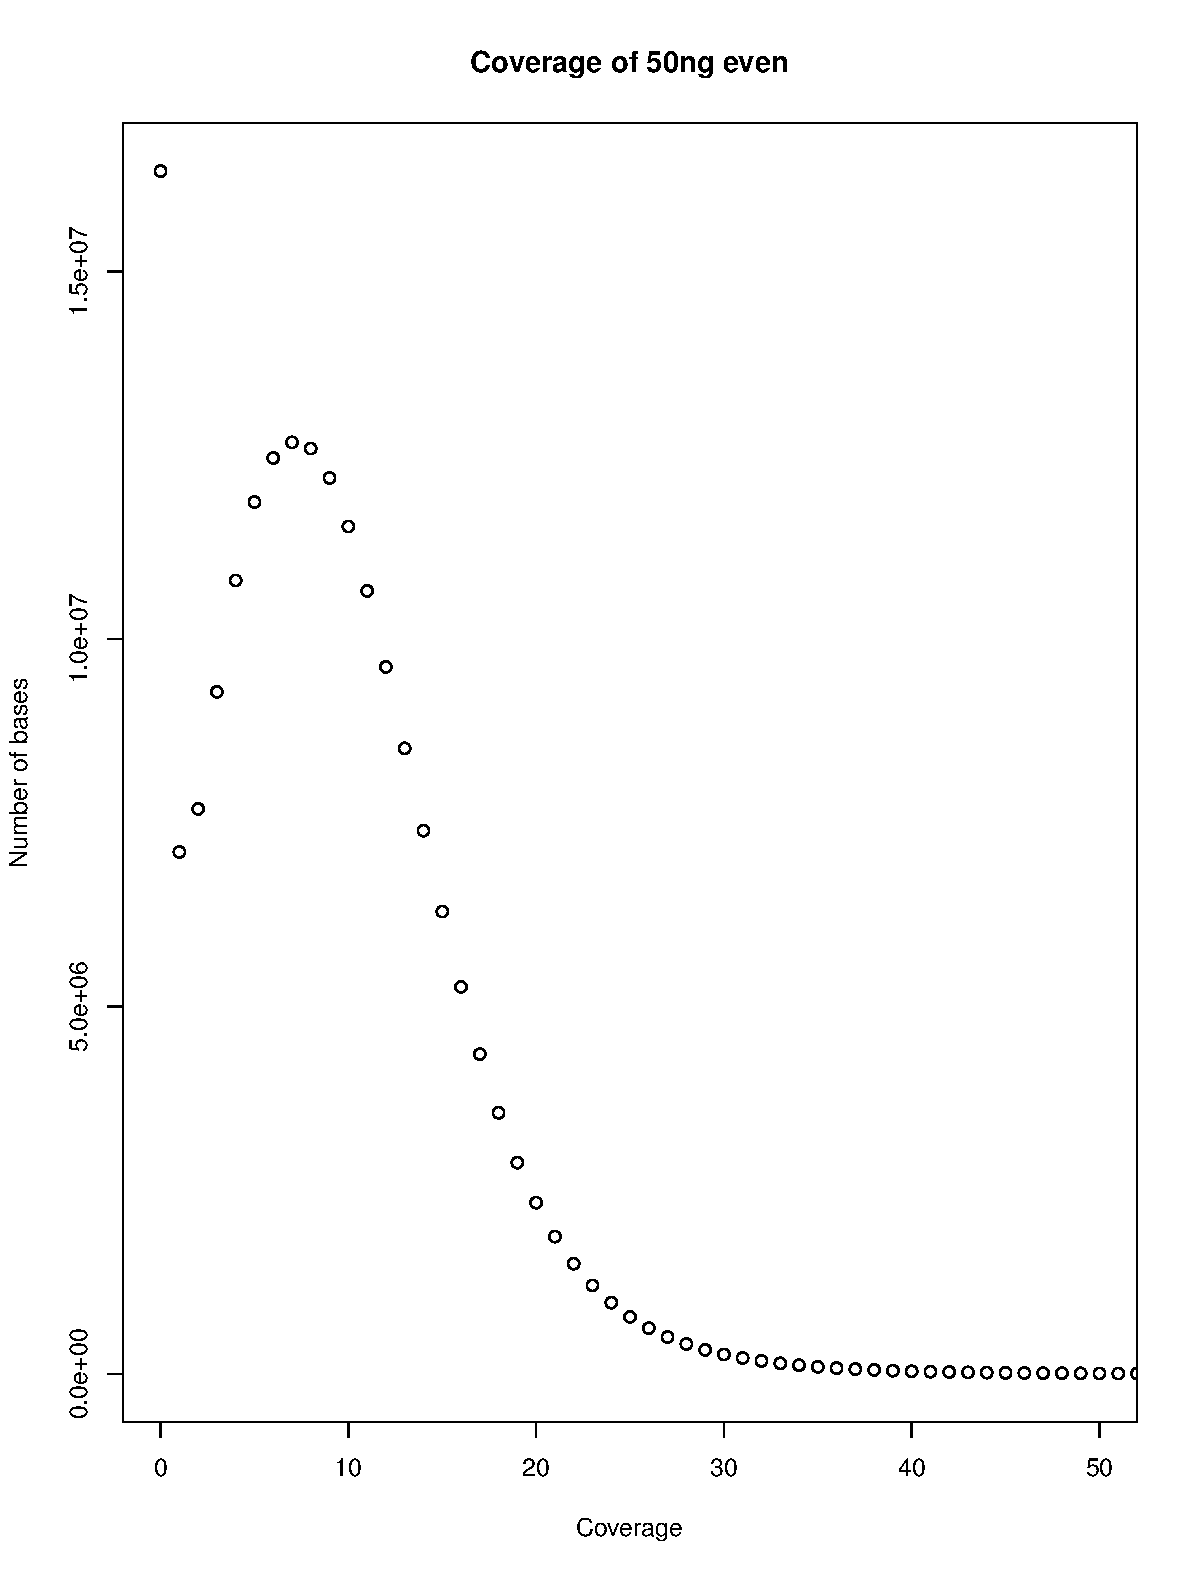
\includegraphics[width=\textwidth]{figures/coverageperbase-50ng_even.pdf}
  \caption{Coverage of 50ng even}
  \label{fig:coverage50ngeven}
\end{figure}
\begin{figure}[ht!]
  \centering
    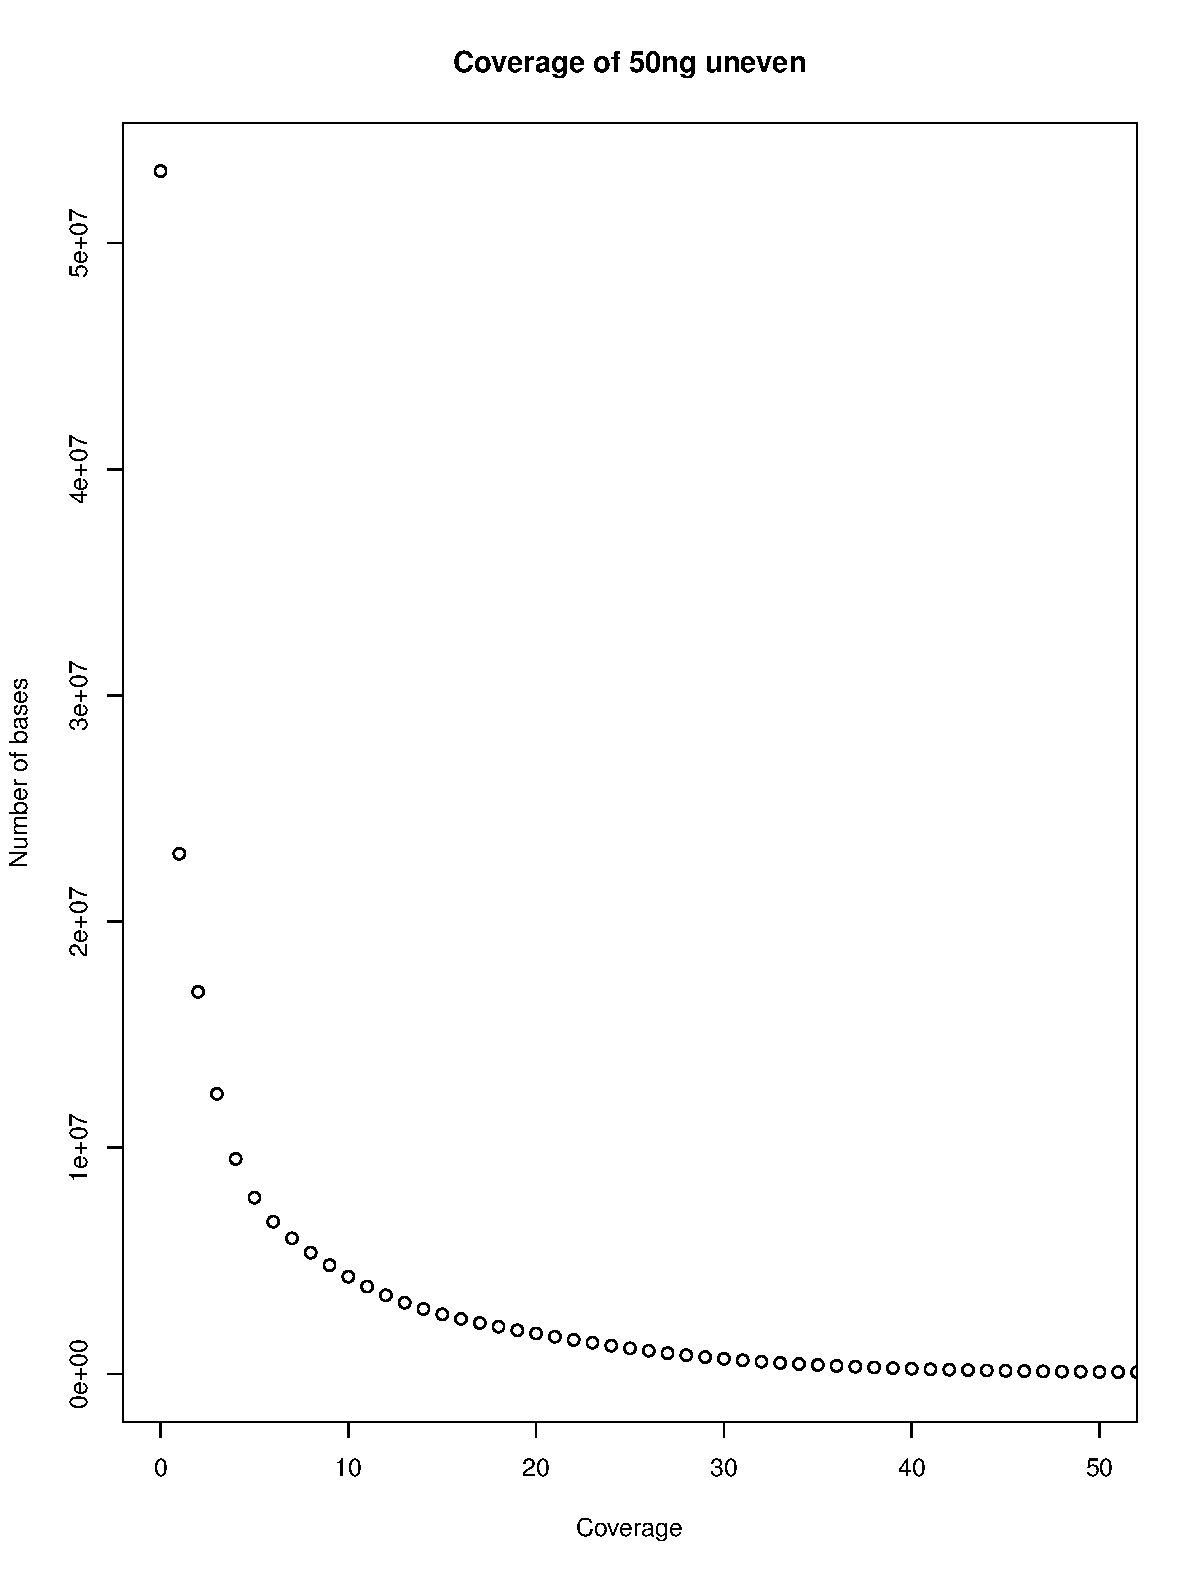
\includegraphics[width=\textwidth]{figures/coverageperbase-50ng_unbalanced.pdf}
  \caption{Coverage of 50ng uneven}
  \label{fig:coverage50nguneven}
\end{figure}

The assemblies have been mapped against the reference metagenome using MUMmer
as described in Section \ref{sec:metval}. In Figure
\ref{fig:l50purity50ng_even} a comparison of the assemblies of 50ng even on
purity and L50 can be seen. The upper right corner contains the assembly that
has the least amount of chimericity and the best contig lengths. The assemblies
seem to perform a lot better for smaller $k$. One would expect to find a sweet
spot for $k$ where lowering $k$ would result in more kmer coverage but more
connectivity in the de Bruijn graph and thus possibly impurer or even shorter
contigs. Upping $k$ would reduce coverage too much to increase contig length.
Such a spot is indeed visible for {\em velvetnoscaf},{\em metavelvetnoscaf} and
{\em velvetscaf} in the top left corner although the purity does not decrease
substantially for smaller $k$, whereas the L50 doubles or even triples. The
contig extension seems to be bound by kmer coverage. Another peculiarity on
first sight is that {\em metavelvetnoscaf} seems to perform identically to {\em
velvetscaf}. The results are similar because for both these assemblies the
parameter \verb!-exp_cov auto! was used for \verb!velvetg! and the scaffolding
parameter of Velvet and Meta-Velvet's default parameters apparently don't
improve the assembly. Meta-Velvet does not improve the Velvet assembly, because
it is based on the idea that genomes have different coverage and tries to
follow paths in the graph with identical coverage. Since all genomes have
similar coverage \verb!velvetg -exp_cov auto!  performs equally well as
\verb!meta-velvetg -exp_cov auto!. In a library with uneven genome abundances,
following paths of identical coverage in the graph does improve the assembly
compared to using one expected coverage as can be seen in Figure
\ref{fig:l50purity50ng_uneven}, where assemblies of an unevenly balanced
community are compared. Why only setting the expected coverage and not the
scaffolding of Velvet increases L50 is unclear. For merging the assemblies of
different kmers into one, Newbler outperforms Minimus2 both on purity and on
L50. An even greater L50 length can be acquired by scaffolding afterwards with
Bambus2, which performs exceptionally well. The best assemblies are
acquired by merging Meta-Velvet assemblies with Minimus or Newbler and
scaffolding them with Bambus2. Scaffolding of Meta-Velvet is significantly
worse performing on purity than Bambus2. For the uneven community, the best
assemblies are done by a combination of Meta-Velvet and Bambus2. Merging
contigs before scaffolding is disadvantageous in this case. The distribution of
the points from both Meta-Velvet and Velvet follow a more distorted path
compared to the even community. There seem to be some specific clusters visible
but no explanation for the cause of this behaviour has been found.

\begin{figure}[ht!]
  \centering
    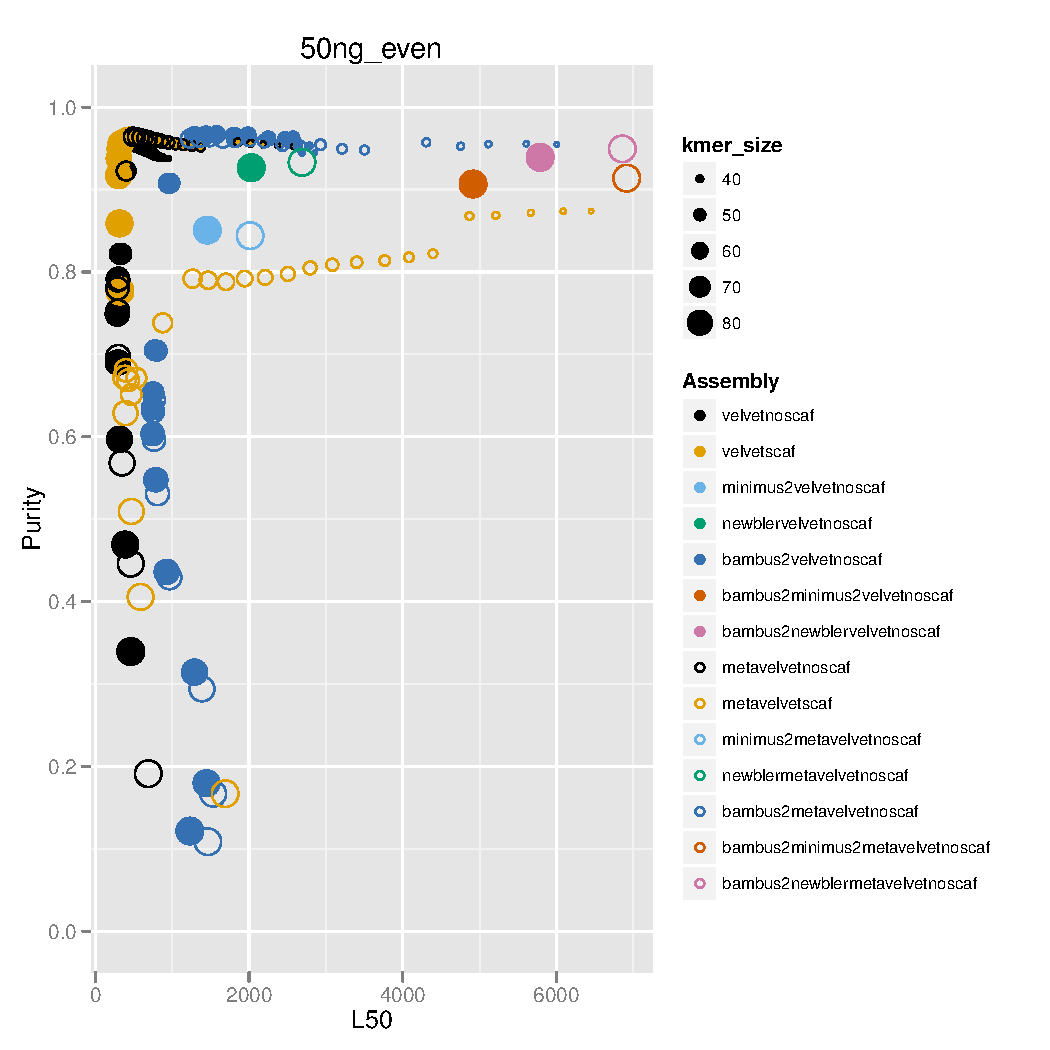
\includegraphics[width=\textwidth]{figures/l50-purity-50ng_even.pdf}
  \caption{L50 versus Purity for 50ng even library. The Velvet assemblies have filled points while the Meta-Velvet assemblies have unfilled points.}
  \label{fig:l50purity50ng_even}
\end{figure}
\begin{figure}[ht!]
  \centering
    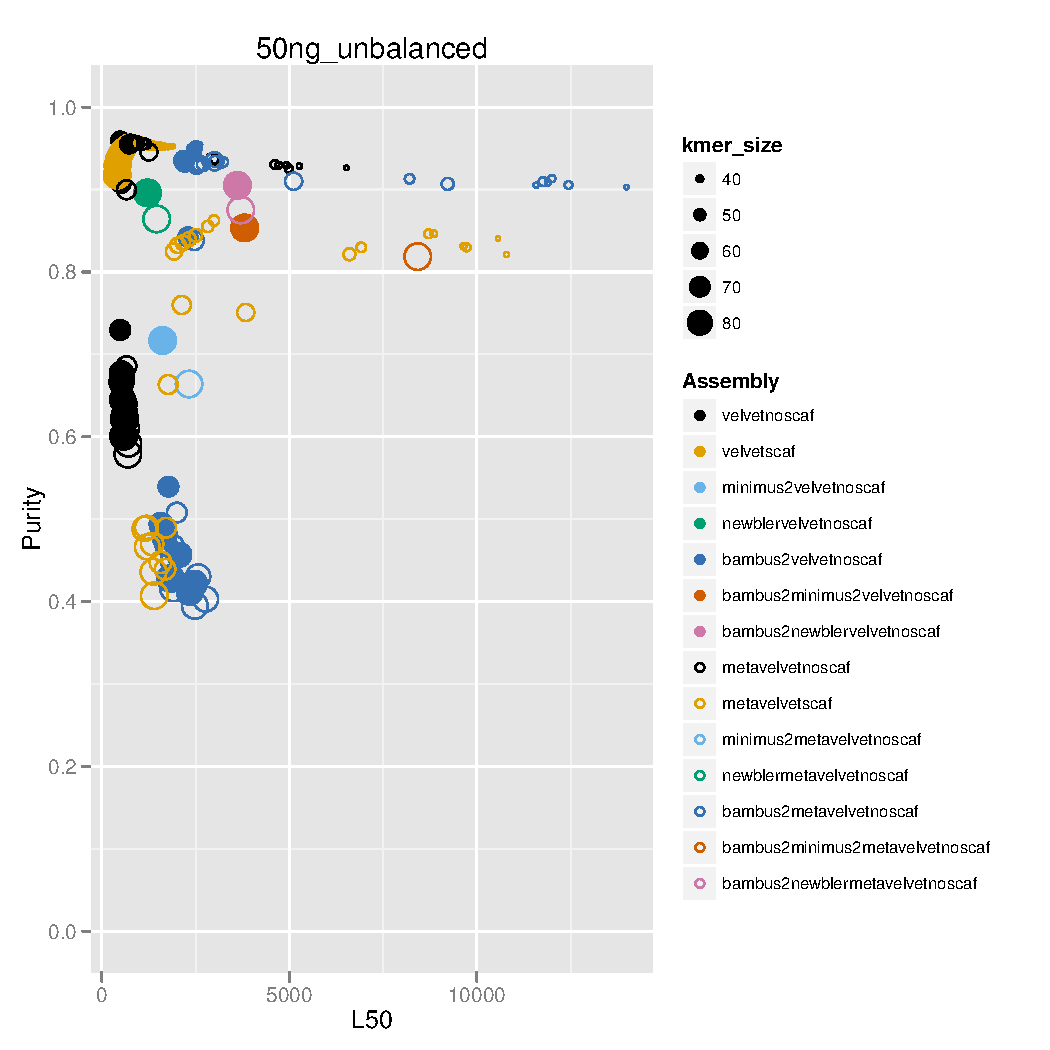
\includegraphics[width=\textwidth]{figures/l50-purity-50ng_unbalanced.pdf}
  \caption{L50 versus Purity for 50ng uneven library. The Velvet assemblies have filled points while the Meta-Velvet assemblies have unfilled points.}
  \label{fig:l50purity50ng_uneven}
\end{figure}


\chapter{Discussion}
Discuss.
%Low coverage libraries
%Future work from presentation

\clearpage
%\bibliographystyle{report.bst}
\bibliographystyle{plainnat}
\bibliography{report}

% Supplementary section
\appendix
\clearpage
\pagestyle{empty}
\begin{landscape}
\footnotesize
\begin{table}[htbp]
\begin{tabular}{|l|r|p{10cm}|}
\hline
Program & Version & URL \\ \hline
sickle & commit 2013-4-3 e435598aa6bbb74b3254d2884a9dea1b0639d464 & \url{https://github.com/najoshi/sickle} \\ \hline
Velvet & 1.2.01 & \url{https://github.com/dzerbino/velvet/commit/5d5b636c52e94fde745cb8bf753ffa134126e04d} \\ \hline
Meta-Velvet & 1.2.01 &  \\ \hline
Minimus2 & Amos commit 2012-3-6 & \url{http://amos.git.sourceforge.net/git/gitweb.cgi?p=amos/amos;a=commit;h=7c70d6c36dba244ae0b266fc52a5206ab202a36c} \\ \hline
Newbler & RunAssembly 2.6 (20110517\_1502) &  \\ \hline
MUMmer & 3.23 & \url{http://sourceforge.net/projects/mummer/files/mummer/3.23/MUMmer3.23.tar.gz/download} \\ \hline
CD-HIT & 4.5.7 & \\ \hline
Picard & 1.77 & \\ \hline
bwa & 0.6.1-r104 & \\ \hline
Bambus2 & Amos commit 2012-3-6 & \url{http://amos.git.sourceforge.net/git/gitweb.cgi?p=amos/amos;a=commit;h=7c70d6c36dba244ae0b266fc52a5206ab202a36c} \\ \hline
samtoafg & Amos commit 2012-3-6 & \url{http://amos.git.sourceforge.net/git/gitweb.cgi?p=amos/amos;a=commit;h=7c70d6c36dba244ae0b266fc52a5206ab202a36c} \\ \hline 
Ray & 2.1.0 & \url{http://denovoassembler.sourceforge.net/}
\end{tabular}
\caption{Program versions used for the analysis}
\label{tab:programversions}
\end{table}
\end{landscape}


\clearpage
\begin{landscape}
\begin{table}[h!]
\begin{tabular}{|l|p{17cm}|}
\hline
Assembly strategy name & Program Parameters\\
\hline
velvetnoscaf & Run \verb!velveth $dir 31,84,2 -fastq -shortPaired $pairs.fastq! and run \verb!velvetg -scaffolding no! on the resulting directories.\\\hline
velvetscaf & Run \verb!velveth $dir 31,84,2 -fastq -shortPaired $pairs.fastq! and run \verb!velvetg -scaffolding yes -exp_cov auto! on the resulting directories.\\\hline
metavelvetnoscaf & Run \verb!velveth $dir 31,84,2 -fastq -shortPaired $pairs.fastq! and run \verb!velvetg -scaffolding no -exp_cov auto -read_trkg yes && -scaffolding no! on the resulting directories.\\\hline
metavelvetscaf & Run \verb!velveth $dir 31,84,2 -fastq -shortPaired $pairs.fastq! and run \verb!velvetg -scaffolding no -exp_cov auto -read_trkg yes && -scaffolding yes! on the resulting directories.\\\hline
raynoscaf & Run \verb!Ray -k $kmersize -i $pairs.fastq -o output_dir!.\\\hline
minimus2* & Concatenate contigs larger than 200 and run \newline\verb!cd-hit-est -c 0.99 -i $concat.fasta -o $derep.fasta! to remove similar sequences. Run \verb!toAmos -s $derep.fasta -o $derep.afg! followed by \verb!minimus2 $derep!. From \url{http://ged.msu.edu/angus/metag-assembly-2011/velvet-multik.html} \\\hline
newbler* & Cut all contigs up in chunks of 1999 bases with an overlap of 1900 bases and run\newline \verb!runAssembly -o $dir $cut-up-contigs.fasta!. From \cite{Luo22347999}. \\\hline
bambus2* & Map paired reads with \verb!bwa! using default parameters to contigs and remove duplicate reads with \verb!MarkDuplicates!. Run \verb!samtoafg! to convert to afg, import to Amos bnk with \verb!bank-transact! and finally run \verb!goBambus2!.\\\hline
\hline
\end{tabular}
\caption{Program parameters per assembly strategy.}
\label{tab:asmstratparameters}
\end{table}
\end{landscape}

\clearpage
\begin{landscape}
\begin{center}
\footnotesize
\begin{longtable}{|r|l|c|l|l|l|}
\caption{Mock community}\label{tab:mock}\\
\hline
No & Genome Name & Genome Size (bp) & Domain & Phylum & Class \\

\hline
\endfirsthead
\multicolumn{6}{c}%
{{\bfseries \tablename\ \thetable{} Mock Community -- continued from previous page}} \\
\hline
No & Genome Name & Genome Size (bp) & Domain & Phylum & Class \\
\hline
\endhead

\hline \multicolumn{6}{|r|}{{Continued on next page}} \\ \hline
\endfoot

\hline 
\endlastfoot
1 & Acidobacterium capsulatum ATCC 51196 & 4127356 & Bacteria & Acidobacteria & Acidobacteriae \\
2 & Akkermansia muciniphila ATCC BAA-835 & 2664102 & Bacteria & Verrucomicrobia & Verrucomicrobiae \\
3 & Anaerocellum thermophilum Z-1320, DSM 6725 & 2919718 & Bacteria & Firmicutes & Clostridia \\
4 & Bacteroides thetaiotaomicron VPI-5482 & 6293399 & Bacteria & Bacteroidetes & Bacteroidia \\
5 & Bacteroides vulgatus ATCC 8482 & 5163189 & Bacteria & Bacteroidetes & Bacteroidia \\
6 & Bordetella bronchiseptica RB50 & 5339179 & Bacteria & Proteobacteria & Betaproteobacteria \\
7 & Burkholderia xenovorans LB400 & 973113 & Bacteria & Proteobacteria & Betaproteobacteria \\
8 & Caldicellulosiruptor saccharolyticus DSM 8903 & 2970275 & Bacteria & Firmicutes & Clostridia \\
9 & Chlorobaculum tepidum TLS & 2154946 & Bacteria & Chlorobi & Chlorobia \\
10 & Chlorobium limicola DSM 245 & 2763181 & Bacteria & Chlorobi & Chlorobia \\
11 & Chlorobium phaeobacteroides DSM 266 & 3133902 & Bacteria & Chlorobi & Chlorobia \\
12 & Chlorobium phaeovibrioides DSM 265 & 1966858 & Bacteria & Chlorobi & Chlorobia \\
13 & Chloroflexus aurantiacus J-10-fl & 5258541 & Bacteria & Chloroflexi & Chloroflexi \\
14 & Clostridium thermocellum ATCC 27405 & 3843301 & Bacteria & Firmicutes & Clostridia \\
15 & Deinococcus radiodurans R1 & 3284156 & Bacteria & Thermi & Deinococci \\
16 & Desulfovibrio desulfuricans desulfuricans ATCC 27774 & 2873437 & Bacteria & Proteobacteria & Deltaproteobacteria \\
17 & Desulfovibrio piger ATCC 29098 & 2826240 & Bacteria & Proteobacteria & Deltaproteobacteria \\
18 & Dictyoglomus turgidum DSM 6724 & 1855560 & Bacteria & Dictyoglomi & Dictyoglomia \\
19 & Enterococcus faecalis V583 & 3359974 & Bacteria & Firmicutes & Bacilli \\
20 & Fusobacterium nucleatum nucleatum ATCC 25586 & 2174500 & Bacteria & Fusobacteria & Fusobacteria \\
21 & Gemmatimonas aurantiaca T-27T & 4636964 & Bacteria & Gemmatimonadetes & Gemmatimonadetes \\
22 & Herpetosiphon aurantiacus ATCC 23779 & 6785430 & Bacteria & Chloroflexi & Chloroflexi \\
23 & Hydrogenobaculum sp. Y04AAS1 & 1559514 & Bacteria & Aquificae & Aquificae \\
24 & Leptothrix cholodnii SP-6 & 4909403 & Bacteria & Proteobacteria & Betaproteobacteria \\
25 & Nitrosomonas europaea ATCC 19718 & 2812094 & Bacteria & Proteobacteria & Betaproteobacteria \\
26 & Nostoc sp. PCC 7120 & 7211789 & Bacteria & Cyanobacteria & unclassified \\
27 & Pelodictyon phaeoclathratiforme BU-1 & 3018238 & Bacteria & Chlorobi & Chlorobia \\
28 & Persephonella marina EX-H1 & 2467104 & Bacteria & Aquificae & Aquificae \\
29 & Porphyromonas gingivalis ATCC 33277 & 2354886 & Bacteria & Bacteroidetes & Bacteroidia \\
30 & Rhodopirellula baltica SH 1 & 7145576 & Bacteria & Planctomycetes & Planctomycetacia \\
31 & Rhodospirillum rubrum ATCC 11170 & 4406557 & Bacteria & Proteobacteria & Alphaproteobacteria \\
32 & Ruegeria pomeroyi DSS-3 & 4601053 & Bacteria & Proteobacteria & Alphaproteobacteria \\
33 & Salinispora arenicola CNS-205 & 5786361 & Bacteria & Actinobacteria & Actinobacteria \\
34 & Salinispora tropica CNB-440 & 5183331 & Bacteria & Actinobacteria & Actinobacteria \\
35 & Shewanella baltica OS185 & 5312910 & Bacteria & Proteobacteria & Gammaproteobacteria \\
36 & Shewanella baltica OS223 & 5358884 & Bacteria & Proteobacteria & Gammaproteobacteria \\
37 & Sulfitobacter sp. EE-36 & 3547243 & Bacteria & Proteobacteria & Alphaproteobacteria \\
38 & Sulfitobacter sp. NAS-14.1 & 4002069 & Bacteria & Proteobacteria & Alphaproteobacteria \\
39 & Sulfurihydrogenibium sp. YO3AOP1 & 1838442 & Bacteria & Aquificae & Aquificae \\
40 & Sulfurihydrogenibium yellowstonense SS-5 & 1534471 & Bacteria & Aquificae & Aquificae \\
41 & Thermoanaerobacter pseudethanolicus ATCC 33223 & 2362816 & Bacteria & Firmicutes & Clostridia \\
42 & Thermotoga neapolitana DSM 4359 & 1884562 & Bacteria & Thermotogae & Thermotogae \\
43 & Thermotoga petrophila RKU-1 & 1824357 & Bacteria & Thermotogae & Thermotogae \\
44 & Thermotoga sp. RQ2 & 1877693 & Bacteria & Thermotogae & Thermotogae \\
45 & Thermus thermophilus HB8 & 2116056 & Bacteria & Thermi & Thermi \\
46 & Treponema denticola ATCC 35405 & 2843201 & Bacteria & Spirochaetes & Spirochaetes \\
47 & Wolinella succinogenes DSM 1740 & 2110355 & Bacteria & Proteobacteria & Epsilonproteobacteria \\
48 & Zymomonas mobilis mobilis ZM4 & 2223497 & Bacteria & Proteobacteria & Alphaproteobacteria \\
49 & Archaeoglobus fulgidus DSM 4304 & 2178400 & Archaea & Euryarchaeota & Archaeoglobi \\
50 & Ignicoccus hospitalis KIN4/I & 1297538 & Archaea & Crenarchaeota & Thermoprotei \\
51 & Methanocaldococcus jannaschii DSM 2661 & 1 664 970 & Archaea & Euryarchaeota & Methanococci \\
52 & Methanococcus maripaludis C5 & 1 780 761 & Archaea & Euryarchaeota & Methanococci \\
53 & Methanococcus maripaludis S2 & 1 661 137 & Archaea & Euryarchaeota & Methanococci \\
54 & Nanoarchaeum equitans Kin4-M & 490 885 & Archaea & Nanoarchaeota & Nanoarchaea \\
55 & Pyrobaculum aerophilum IM2 & 2 222 430 & Archaea & Crenarchaeota & Thermoprotei \\
56 & Pyrobaculum calidifontis JCM 11548 & 2 009 313 & Archaea & Crenarchaeota & Thermoprotei \\
57 & Pyrococcus horikoshii OT3 & 1 738 505 & Archaea & Euryarchaeota & Thermococci \\
58 & Sulfolobus tokodaii 7(S311) & 2 694 756 & Archaea & Crenarchaeota & Thermoprotei \\
59 & Treponema vincentii I & 2512734 & Bacteria & Spirochaetes & Spirochaetia \\
%60 & Erwinia chrysanthemi & 3909000 & Bacteria & Proteobacteria; & Gammaproteobacteria \\
\end{longtable}
\end{center}
\end{landscape}


\end{document}
